\documentclass[twocolumn,prl,showpacs,superscriptaddress]{revtex4-1}   % use preprint or twocolumn
%\usepackage{geometry}                % See geometry.pdf to learn the layout options. There are lots.
%\geometry{letterpaper}                   % ... or a4paper or a5paper or ...
%\geometry{landscape}                % Activate for for rotated page geometry
%\usepackage[parfill]{parskip}    % Activate to begin paragraphs with an empty line rather than an indent
\usepackage{graphicx}
\usepackage{amsmath}
\usepackage{amssymb}
\usepackage{epstopdf}
\usepackage{dcolumn}% Align table columns on decimal point
\usepackage{bm}% bold math
\usepackage{verbatim}
\usepackage{amsfonts}
\usepackage{cancel}
\usepackage[utf8]{inputenc}
\usepackage{graphicx}
\usepackage{setspace}
\usepackage[export]{adjustbox}

\DeclareGraphicsRule{.tif}{png}{.png}{`convert #1 `dirname #1`/`basename #1 .tif`.png}

\newcommand{\proofend}{\mbox{ }\hfill$\Box$\\}
\newcommand{\ddf}[2]{\frac{\mathrm{d} #1}{\mathrm{d} #2}}
\newcommand{\pdf}[2]{\frac{\partial #1}{\partial #2}}
\newcommand{\ee}[1]{\cdot 10^{ #1}}
\newcommand{\bra}[1]{\left\langle #1 \right|}
\newcommand{\ket}[1]{\left| #1 \right\rangle}
\newcommand{\brakett}[3]{\left\langle #1 \right|#2\left| #3 \right\rangle}
\newcommand{\braket}[2]{\left\langle #1 \right|\left. #2 \right\rangle}
\newcommand{\trace}[1]{\mathrm{Tr}\left(#1\right)}
\newcommand{\abs}[1]{\left|#1\right|}
\newcommand{\figref}[1]{Fig. \ref{#1}}
\newcommand{\eqnref}[1]{Eqn. \eqref{#1}}

\newcommand{\ak}{\alpha_{\textrm{K}}}
\newcommand{\arb}{\alpha_{\textrm{Rb}}}
\newcommand{\acs}{\alpha_{\textrm{Cs}}}
\newcommand{\acore}{\alpha_{\textrm{core}}}
\newcommand{\atail}{\alpha_{\textrm{tail}}}

\newcommand{\polK}{42.97(2)(8)}
\newcommand{\polRb}{47.44(3)(9)}
\newcommand{\polCs}{59.45(3)(11)}
\newcommand{\polKSysOnly}{42.97(8)}
\newcommand{\polRbSysOnly}{47.44(9)}
\newcommand{\polCsSysOnly}{59.45(11)}

\newcommand{\ratRbK}{1.1040(9)}
\newcommand{\ratCsK}{1.3835(9)}
\newcommand{\ratCsRb}{1.2532(10)}

% obselete
\newcommand{\sigv}{ASDFASDFASDF}
\newcommand{\sigr}{ASDFASDFASDFA}

\newcommand{\Omegalab}{\Omega_{\mathrm{lab},y}}

\newcommand{\dphisep}{\Delta\Phi_{\mathrm{sep}}}
\newcommand{\dphisepj}{\Delta\Phi_{\mathrm{sep},j}}

\newcommand{\dphisag}{\Delta\Phi_{\mathrm{sag}}}
\newcommand{\dphiaccel}{\Delta\Phi_{\mathrm{accel}}}

\newcommand{\cenv}{C_{\mathrm{env}}}

\newcommand{\rcs}{R_{\mathrm{Cs}}}

\newcommand{\etal}{\textit{et al.}}
\newcommand{\etalspace}{\textit{et al. }}

\newcommand{\AAA}{\mathrm{\AA}}




\begin{document}

%\title{Improved Absolute and Ratio Measurements of Ground-State Polarizabilities of Cs, Rb, and K using Atom Interferometry}
\title{Measurements of the Ground-State Polarizabilities of Cs, Rb, and K using Atom Interferometry}

\affiliation{Department of Physics, University of Arizona, Tucson, AZ 85721}
\affiliation{College of Optical Sciences, University of Arizona, Tucson, AZ 85721}
\author{Maxwell D. Gregoire}
\affiliation{Department of Physics, University of Arizona, Tucson, AZ 85721}
\author{Ivan Hromada}
\affiliation{Department of Physics, University of Arizona, Tucson, AZ 85721}
\author{William F. Holmgren}
\affiliation{Department of Physics, University of Arizona, Tucson, AZ 85721}
\author{Raisa Trubko}
\affiliation{College of Optical Sciences, University of Arizona, Tucson, AZ 85721}
\author{Alexander D. Cronin}
\affiliation{Department of Physics, University of Arizona, Tucson, AZ 85721}
\affiliation{College of Optical Sciences, University of Arizona, Tucson, AZ 85721}
\email{cronin@physics.arizona.edu}
\homepage{http://www.atomwave.org}

\date{\today}





\begin{abstract}
We measured the ground-state static electric-dipole polarizabilities of Cs, Rb, and K atoms using a three-nanograting Mach-Zehnder atom beam interferometer. Our measurements provide benchmark tests for atomic structure calculations and thus test the underlying theory used to interpret atomic parity non-conservations experiments. We measured $\acs = 4\pi\epsilon_0 \times \polCsSysOnly \AAA^3$, $\arb = 4\pi\epsilon_0 \times \polRbSysOnly \AAA^3$, and $\ak = 4\pi\epsilon_0 \times \polKSysOnly \AAA^3$. We report ratios of polarizabilities $\acs/\arb = \ratCsRb$, $\acs/\ak = \ratCsK$, and $\arb/\ak = \ratRbK$ with smaller fractional uncertainty because several sources of systematic error are common mode. 
Since Cs atom beams have shorter de Broglie wavelengths, we developed measurement methods that do not require resolved atom diffraction patterns.
Specifically, we used phase choppers to measure atomic beam velocity distributions, and electric field gradients to induce atom interference fringe phase shifts proportional to atomic polarizability.
\end{abstract}





\maketitle



\begin{figure*}
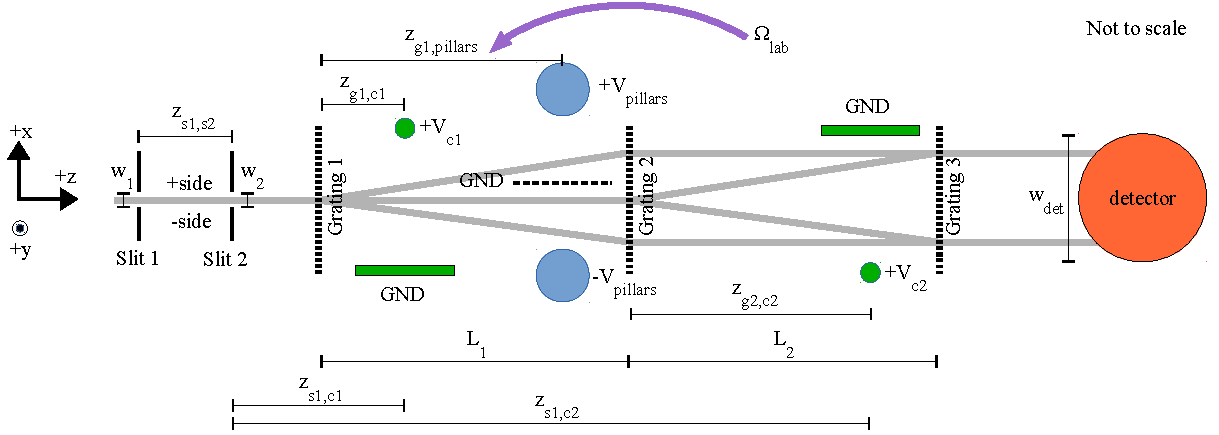
\includegraphics[width=\linewidth,keepaspectratio]{IFM_diagram1.pdf}
\caption{\label{IFMDiagram}(Color online) Diagram of the atom interferometry apparatus. The supersonic atom beam is collimated by two slits, s1 and s2, before entering the three-grating Mach-Zehnder interferometer. 
The gratings, g1, g2, and g3, are spaced longitudinally such that $L_1 = L_2$ so that an interference pattern forms at the position of the third grating.
Due to the rotation of the Earth, the lab has a rotation rate about the vertical axis of $\Omegalab = 38.88\mu$rad/s. 
The pair of blue circles represents oppositely-charged cylindrical electrodes (extending perpendicular to the page), that form an effective ground plane between them. The electric field from these electrodes polarizes the atoms and thereby shift the interference pattern. 
The phase choppers are represented by the two groups of one green circle and one green rectangle; each phase chopper is a charged wire next to a grounded plane. The geometry terms relevant to the pillars and phase choppers are displayed in \figref{EDiagram} and discussed in section II.a. Dimensions are given in Table \ref{tableDimensions}.}
\end{figure*}

\section{I. Introduction}

We measured the static electric-dipole polarizabilities of K, Rb, and Cs atoms with $<0.2\%$ uncertainty using a Mach-Zehnder three-grating atom interferometer \cite{Berman1997,Cronin2009} with an electric field gradient interaction region. We used the same apparatus for all three atomic species, so we can also report polarizability ratios with $<0.1\%$ uncertainty because many sources of uncertainty are correlated between measurements of different atoms. 

Measuring alkali static polarizabilities as a means of testing atomic 
structure calculations has been of interest to the physics community since
1934 \cite{Scheffers1934}, and has been
accomplished using deflection \cite{Scheffers1934,Chamberlain1963,Hall1974}, the E-H gradient
balance technique \cite{Salop1961,Molof1974}, and, most recently, time-of-flight measurements of atoms in a fountain \cite{Amini2003} and atom interferometry 
\cite{Ekstrom1995,Miffre2006,Holmgren2010}.
Our measurements serve as benchmark tests for ab initio calculations of electric dipole transition matrix elements. This is important because there are many competing methods that attempt to calculate these matrix elements of many-electron atoms in a reasonable amount of computing time \cite{Mitroy2010}. 

We also compare our measurements to polarizability values of comparable uncertainty deduced from studies of atomic lifetimes, Feshbach resonances, and photoassociation specroscopy. Then we analyze our measurements to report the Cs $6p_{1/2}$ and $6p_{3/2}$ state lifetimes, Rb $5p_{1/2}$ and $5p_{3/2}$ state lifetimes, and K $4p_{1/2}$ and $4p_{3/2}$ state lifetimes, as well as the associated principal electric dipole matrix elements, oscillator strengths, and line strengths. 
We also use our $\acs$ measurement to report the Cs van der Waals $C_6$ coefficient,
and we combine our measurements with recent measurements of 
Cs $\alpha_{6p_{1/2}} - \alpha_{6s_{1/2}}$,
Rb $\alpha_{5p_{1/2}} - \alpha_{5s_{1/2}}$, and
K $\alpha_{4p_{1/2}} - \alpha_{4s_{1/2}}$ to report excited state polarizabilities.

Testing Cs atomic structure calculations by measuring $\acs$ is particularly important for parity non-conservation (PNC) research, which is important for placing constraints on beyond-the-standard-model physics. The coupling strength, $E_{\mathrm{PNC}}$, of $Z^0$-mediated interactions between the Cs chiral, valence electron and nuclear neutrons can be written in terms of the electric dipole transition matrix elements and the nuclear weak charge parameter $Q_W$. Researchers can use atomic structure calculations to deduce a value of $Q_W$ from an $E_{\mathrm{PNC}}$ measurement \cite{Cho1997} to compare to the $Q_W$ predicted by the standard model \cite{Bouchiat1999,Dzuba2012}. Our measurement of $\acs$ tests the methods used to calculate the relevant matrix elements and provides a fairly direct benchmark for the $\brakett{6s_{1/2}}{\hat{D}}{6p_{1/2}}$ matrix element, one of the most dominant terms in the expression for $E_{\mathrm{PNC}}$.

To our knowledge, this is the first time atom interferometry has been used to measure Cs polarizability. Measuring polarizability by the method described here requires precise measurement of our atom beam's velocity distribution. Because it is challenging to obtain resolved diffraction with a 1500 m/s Cs beam,we did not measure its velocity using diffraction as was done by Ekstrom \etalspace and Holmgren \etalspace \cite{Ekstrom1995,Holmgren2010}. We overcame this obstacle by measuring the beam velocity using phase choppers,  invented by Tony Roberts and David Pritchard \cite{Roberts2002,Roberts2004} as a successor to mechanical choppers.
Phase choppers, described in Section II, are a pair of electric field gradients turned on and off at varying frequencies that modify the interference pattern's contrast based on the beam velocity distribution. 

We improved upon the accuracy of Holmgren \etal's work by redesigning the configuration of electrodes used to polarize the atoms in our beams. We also advanced our analysis by considering the finite thickness and divergence of the beam, the finite width of the detector, and the effects of de Broglie wavefront curvature induced by our electrodes, as discussed by Hromada \etalspace \cite{Hromada2014}.

%H. Scheffers and J. Stark, Phys. Z. 35, 625 (1934)

\section{II. Apparatus Description and Error Analysis}

\begingroup
\begin{table}
\caption{\label{tableDimensions}List of apparatus dimensions, which are described in \figref{IFMDiagram} and \figref{EDiagram}. Dimensions with no quoted uncertainty have uncertainty much less than what would be significant to our analysis.}
\begin{center}
\begin{tabular}{l l}
\hline\hline
$z_{\mathrm{s1,s2}}$ & 860 mm \\
$z_{\mathrm{g1,pillars}}$ & (833.5 $\pm$ 0.25) mm \\
$z_{\mathrm{g1,c1}}$ & 269.7 mm \\
$z_{\mathrm{s2,c1}}$ & 100 mm \\
$z_{\mathrm{g2,c2}}$ & 598 mm \\
$z_{\mathrm{c1,c2}}$ & (1269.3 $\pm$ 0.25) mm \\
$L_1$ & 940 mm \\
$L_2$ & 940 mm \\
$w_1$ & (30 $\pm$ 6) $\mu$m \\
$w_2$ & (40 $\pm$ 6) $\mu$m \\
$w_{\mathrm{det}}$ & (100 $\pm$ 20) $\mu$m \\ 
$a_{\mathrm{pillars}}$ & (3999.7 $\pm$ 1.0) $\mu$m \\
$R_{\mathrm{pillars}}$ & (6350 $\pm$ 1) $\mu$m \\
$a_{c1}$ & (986 $\pm$ 25) $\mu$m \\
$R_{c1}$ & 785.5 $\mu$m \\
$a_{c2}$ & (893 $\pm$ 25) $\mu$m \\
$R_{c2}$ & 785.5 $\mu$m \\
\hline\hline
\end{tabular}
\end{center}
\end{table}
\endgroup

A schematic diagram of the three-grating Mach-Zehnder atom beam interferometer we use to make our measurements is shown in \figref{IFMDiagram}. 
A mix of 85\% He and 15\% Ar gas carries Cs, Rb, or K vapor through a small nozzle to generate a supersonic atom beam \cite{Scoles} \cite{Ekstrom1993}. 
The atom beam passes through two collimating slits and diffracts through three silicon nitride nano-gratings, each with period $d_g = 100$ nm.
The first two gratings form a 100nm-period interference pattern at the position of the third grating, which acts as a mask for that interference pattern. 
The method of observing fringes is described in detail in \cite{Kokorowski2001}: we scan the second grating in the $\pm x$ direction and observe the flux admitted through the third grating in order to determine the interference pattern's contrast and phase.
We detect the atoms with a 100 $\mu$m-wide platinum wire Langmuir-Taylor detector \cite{Delhuille2002}.

In the rest of Section II we describe how we measure the atoms' velocity distribution and the polarizability.
We measure static polarizability $\alpha$ with a non-uniform electric field created by two oppositely charged pillars parallel with the $y$ axis, indicated in blue in \figref{IFMDiagram}. The pillars' electric field shifts the phase by an amount roughly proportional to $\alpha/v_0^2$, where $v_0$ is the atoms' mean velocity. We measure $v_0$ using phase choppers, which are charged wires parallel with the $y$ axis held near and parallel to grounded planes, indicated in green in \figref{IFMDiagram}.
Section II.a. describes how the electric field geoemtry of both the phase choppers and the pillars causes a differential phase shift. Then, section II.b. describes how we use the phase choppers to measure the velocity distribution, and section II.c. describes how we use the pillars to measure $\alpha$. Section II.d. discusses how we apply our knowledge of the velocity distribution to analysis of the data taken with the pillars.


\subsection{II.a. Phase Shifts with Cylindrical Electrodes}

\begin{figure}
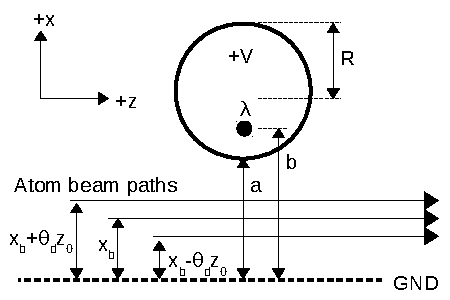
\includegraphics[width=\linewidth,keepaspectratio]{EDiagram1.pdf}
\caption{\label{EDiagram}Diagram showing the dimensions that describe the static electric fields created by the pillars and by the phase choppers. The circle represents the cross-section of a metal pillar or charged wire with radius $R$ held at voltage $V$. The GND line represents the ground plane, which may by physical or virtual, a distance $a$ away from the pillar edge. The parameter $b$ is the distance between the ground plane and the effective line charge within the pillar. The atom beam center is a distance $x_b$ away from the ground plane, and the different interferometer arms are separated from their neighbors by a distance $\theta_d z_0$. $a$ and $R$ dimensions for the pillars and phase choppers are given in Table \ref{tableDimensions}.}
\end{figure}

Both the pillars and the phase choppers are described by the geometry shown in \figref{EDiagram}, and have electric fields given by
\begin{align}
	\vec{E}(x,z) = \frac{\lambda}{\pi\epsilon_0}
	\left[	
		\frac{x-b}{(x-b)^2+z^2} - \frac{x+b}{(x+b)^2+z^2}
	\right] \hat{x} \nonumber \\
	+ 
	\left[	
		\frac{z}{(x-b)^2+z^2} - \frac{z}{(x+b)^2+z^2}
	\right] \hat{z}
	\label{EPillars}
\end{align}
The effective line charge density
\begin{align}
	\lambda = 2\pi\epsilon_0V\ln^{-1}
	\left(
		\frac{a+R+b}{a+R-b}
	\right)
	\label{lambda}
\end{align}
exists a distance $b = a\sqrt{1+2R/a}$ away from the ground plane, where $a$ is the distance between the ground plane and the closest cylinder edge, $R$ is the cylinders' radius, and $\hat{x}$ and $\hat{z}$ are shown in \figref{EDiagram}.

The field shifts the atoms' energy by $U_{\mathrm{Stark}} = -\frac{1}{2}\alpha\abs{\vec{E}}^2$.
Since $U_{\mathrm{Stark}} \ll E_{\mathrm{kinetic}}$ in our experiment, we can use the WKB approximation along with the Residue Theorem to compute the total phase accumulated by an atom travelling through the field.
Even though an atom in the beam may be misaligned by an angle of up to $10^{-3}$ with the different fields' ground planes, we can approximate that atoms always travel parallel to the beamline distance $x_b$ away from the ground plane: the effective path length through the field region grows as $1/\cos{\theta} \approx 1+\theta^2$, so a misalignment of $\theta = 10^{-3}$ should increase the phase by only one part in $10^6$, which is insignificant for our purposes. Therefore, the accumulated phase along the path for a single atom is
\begin{align}
	\Phi(v,x) = 
	\frac{1}{\hbar v} \int_{-\infty}^{\infty} \frac{1}{2} \alpha |\vec{E}|^2 dz =	
	\frac{\lambda^2 \alpha}{\pi \epsilon_0^2 \hbar v}
	\left( \frac{b}{b^2-x_b^2} \right)
	\label{accumPhasePillars}
\end{align}

The differential phase shifts for the interferometers on the $j=+1$ and $j=-1$ sides of the beamline (see \figref{IFMDiagram}) are
\begin{align}
	\Delta\Phi_{\vec{E},1}(v,x_b) = \Phi(v, x_b+\theta_d z_0) - \Phi(v, x_b) \nonumber \\
	\Delta\Phi_{\vec{E},-1}(v,x_b) = \Phi(v, x_b) - \Phi(v, x_b-\theta_d z_0)
	\label{deltaPhasePillars}
\end{align}
where $\theta_d z_0$ is the lateral separation between classical paths in the interferometer. 
\figref{phaseShiftExample} shows an example of the interference fringes shifting due to an electric-field-induced differential phase shift.

\begin{figure}
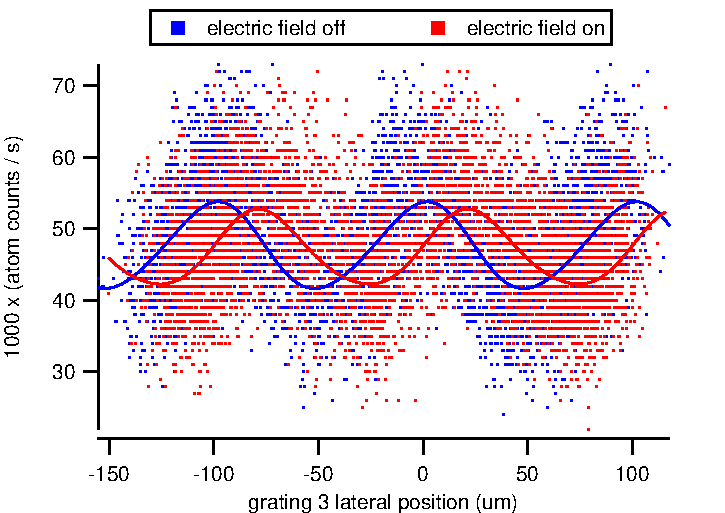
\includegraphics[width=\linewidth,keepaspectratio]{countsVsGratingPos_150420.pdf}
\caption{\label{phaseShiftExample}(Color online) An example of a differential phase shift. The blue and red Cs interference fringes were each observed by moving the third grating in the $\pm x$ direction for 5 seconds. A sine wave was fit to each interference pattern. This figure demonstrates the electric field moving the fringes by about 25 nm, or $d_g/4$, which corresponds to a $\pi/2$ differential phase shift. The fringes observed with the field turned on have slightly lower contrast due to fringe magnification and the longitudinal contrast envelope at the position of grating 3 (see the Velocity Measurement section for details).}
\end{figure}

\subsection{II.b. Velocity Measurement}

The atoms in the beam do not all have the same velocity, so the non-uniform $\vec{E}$ does not apply the same phase shift to each atom.
We observe the average phase and contrast of an ensemble of atoms diffracting to first order on either side of the beamline with velocity distribution $P(v)$. 
We model $P(v)$ as a Gaussian distribution
\begin{align}
	P(v)dv = \frac{v_r}{v_0\sqrt{2\pi}}e^{-\frac{v_r^2(v-v_0)^2}{2v_0^2}}
	\label{PvelGaussian}
\end{align}
where $v_0$ is the mean velocity and $v_r = v_0/\sigma_v$ is a measure of the distribution's sharpness. It is worth noting that the velocity distribution for a supersonic atom beam is better described by
\begin{align}
	P(v)dv = \frac{1}{\sqrt{2\pi}v_0^4(v_r^{-1}+3v_r^{-3})}
	v^3
	e^{-\frac{v_r^2}{2}\left(\frac{v}{v_0}-1\right)^2}
	\label{PvelCubed}
\end{align}
\cite{Berman1997}. However, either distribution can be used in our analysis to parametrize the typical high-$v_0$, high-$v_r$ velocity distributions of our atom beam without changing our polarizability result. Importantly, since $v_0$ and $v_r$ are decoupled in \eqnref{PvelGaussian} and not in \eqnref{PvelCubed}, we choose to use the former for our data analysis in order to simplify the error analysis. 

%Without modelling the beam this way, we would report $\alpha$ 1.5\% too high.

To measure $v_0$ and $v_r$, we use phase choppers. Each phase chopper is a charged wire about 1 mm away from a physical ground plane. Chopper 1 is between the first two gratings and chopper 2 is a distance $z_{c1,c2} = (1269.3 \pm 0.25)$ mm downstream of chopper 1, between the last two gratings (see \figref{IFMDiagram}). The voltage on the wire and the distance between the beam and the ground plane are chosen such that chopper 1 shifts the ensemble's average phase by $+\pi$ and chopper 2 shifts it by $-\pi$. 

When we pulse the choppers on and off at frequency $f_c$, an atom may receive a net phase shift of $\pm\pi$ or $0$ depending on its velocity. Therefore, $v_0$, $v_r$, and $f_c$ determine the fraction of total atoms in the beam which receive a $\pm\pi$ phase shift. This fraction can be quantified by measuring contrast loss $C/C_{\mathrm{ref}}$. To measure $v_0$ and $v_r$, we measure $C/C_{\mathrm{ref}}$ vs $f_c$.

Using phase choppers allows us to measure $v_0$ and $v_r$ for Cs without needing to obtain resolved diffraction. In our earlier work, we measured $v_0$ and $v_r$ by scanning the detector's $x$ position to observe the diffraction pattern through grating 1. However, since the diffraction angle for Cs is so small, we would need a thinner detector wire and thinner collimating slits to resolve diffraction peaks, which would in turn reduce statistical precision.

We have identified a number of systematic errors in our phase chopper velocity distribution measurements, some of which depend on diffraction angle. These errors must be quantified and reduced in order to measure polarizability ratios between atomic species that typically run with different diffraction angles.

In our previous work \cite{Hromada2014}, we documented the systematic errors that would appear if we were to not accurately know $\Delta L = L_1 - L_2$, where $L_1$ is the distance between gratings 1 and 2 and $L_2$ is the distance between gratings 2 and 3. There are two components to this error contribution. The first is that increasing $|\Delta L|$ shifts the interference fringes away from the beamline. We refer to this geometric fringe magnification as the separation phase shift, expressed as
\begin{align}
	\dphisepj = \frac{2\pi}{d_g}
	\left(
		\theta_{inc} + \frac{j}{2}\theta_d
	\right) \Delta L
	\label{phiSep}
\end{align}
where $\theta_{inc}$ is the incident angle of a given atom with deBroglie wavelength $\lambda_{dB}$ on grating 1.
When the fringes on either side of the beamline shift in opposite directions, they interfere less constructively, which results in contrast loss.

The second component of the error is that, as $|\Delta L|$ increases, the longitudinal region at which the atoms' transverse coherence lengths overlap the most is moved away from grating 3, which also results in contrast loss \cite{Champenois1999,McMorran2008}. Furthermore, the electric fields, such as those created by the phase choppers, act as electrostatic lenses that magnify the interference fringes. This magnification also moves the maximal-overlap region longitudinally. Thus the choppers change the contrast simply by turning on, and changing the longitudinal location of the 3rd grating affects how the choppers modify the contrast. Because the ray optics model that we use to describe our interferometer does not assume finite transverse coherence lengths, we define the longitudinal contrast envelope $\cenv$, given by
\begin{align}
	\cenv(t) = e^{-\frac{1}{2} \left( \frac{w_1}{L_1 d_g} \right)^2 (\Delta L - \Delta L_0(t))^2}
	\label{CEnv}
\end{align}
where $w_1$ is the width of the first collimating slit. $\Delta L_0(t)$ is the $\Delta L$ for which the measured contrast is maximum given which phase choppers are on as the atoms pass through them.

Uncertainty in $\Delta L$ contributes more highly to measurements of atom beams with larger $\theta_d$: the effects described by both $\dphisep$ and $\cenv(t)$ are more pronounced when the angles between the paths that converge at grating 3 are greater. Therefore, uncertainty in $\Delta L$ is most significant for $\ak$ measurements and least significant for $\acs$ measurements.

We identified and reduced systematic error by modeling how the collimating slits define the beam's width and divergence and by considering the finite width of the detector, both of which determine how likely it is for atoms of a given velocity to be detected and thus contribute to a measurement of $v_0$. 
We accomplish this by integrating over possible trajectories through the slits (in addition to velocity), parameterized by $x$ positions $x_1$ and $x_2$ from the centers of slits 1 and 2, in order to calculate the average contrast and phase of the atomic ensemble. We also define $D_j(x_1,x_2,v)$, the probability of an atom with velocity $v$ passing through the slits at positions $x_1$ and $x_2$ and diffracting to the $j$ side hitting the detector.
This new model also added elements to the error budget: the widths of the collimating slits ($w_1$ and $w_2$), the detector width ($w_{\mathrm{det}}$), and the offset of the detector in the $x$ direction ($\Delta x_{\mathrm{det}}$) determine how likely it is for atoms with certain velocities to be detected. 

Uncertainties in $w_1$, $w_2$, $w_{\mathrm{det}}$, and $\Delta x_{\mathrm{det}}$ are more significant for beams that are physically wider. 
In K beams, which have higher $\theta_d$ and lower $v_r$ (i.e. a wider velocity distribution), more of the lower-velocity atoms in the distribution miss the detector. Therefore, uncertainties in the aforementioned quanitities have a higher bearing on how we model the average velocity of \underline{detected} atoms. However with Cs beams, which have higher average $\theta_d$ and $v_r$, the detector detects a larger portion of the atoms, rendering the uncertainties in the aforementioned quantities about 10\% as significant as with K beams.
Completely ignoring this component of the analysis causes a systematic increase in measured $v_0$ by 0.05\% and $v_r$ by 10\% for a typical K beam, which corresponds to a 0.15\% error in $\ak$.
 
We find that as $\left|\Delta L\right|$ increases, the measured $v_0$ and $v_r$ become more dependent on the beam width, beam divergence, and detector width. Accordingly, we set $\Delta L = 0$ to reduce contributions to systematic uncertainty in reported $v_0$ from other sources of uncertainty. We begin each day of measurements by setting $\Delta L$ to 0, eliminating the need to consider $\dphisep$. We know that if $\dphisep$ were nonzero, we would see the measured phase change as a function of $\Delta x_{\mathrm{det}}$. We set $\Delta L = 0$ by finding the $\Delta L$ for which the measured phase no longer changes as a function of $\Delta x_{\mathrm{det}}$.

If the interferometer grating bars are significantly non-vertical, it can become necessary to consider the phase shift induced by the component of gravitational acceleration in the plane of the interferometer, which is given by
\begin{align}
	\dphiaccel = \frac{\pi g\sin({\theta_g})(L_1+L_2)^2}{2d_g v^2}
	\label{phiAccel}
\end{align}
where $\theta_g$ is the tilt of the grating bars with respect to vertical. 
Our interferometer's $|\theta_g|$ never exceeded 2.3 mrad, which means that neglecting this portion of the analysis would cause us to report $v_0$ incorrectly by up to 0.015\% and $v_r$ incorrectly by up to 0.25\%.

Taking all these effects into account, our more complete model for contrast loss as a function of chopping frequency is
\begin{align}
	\frac{C}{C_{\mathrm{ref}}}(f_c) = 
	\left|
		\frac{1}{2} \sum_{j=-1,1}
		f_c \int_{t=0}^{1/f_c} 
		\int_{x_1=w_1/2}^{w_1/2}
		\int_{x_2=w_2/2}^{w_2/2}
		\int_{v=0}^{\infty}           
		\right. \nonumber \\
		P(v)
		D_j(x_1, x_2, v)
		\cenv(t)                   
		\nonumber \\ \times
		e^{i\left( \Delta\Phi_{c1,j}(v,x_1,x_2)\Theta\left(t-\frac{1}{2f_c}\right) + \Delta\Phi_{c2,j}(v,x_1,x_2)\Theta\left(t-\frac{z_{c1,c2}}{v}-\frac{1}{2f_c}\right) \right)}
		\nonumber \\ \times \left.
		e^{i( \dphisepj(v,x_1,x_2) + \dphiaccel(v) + \dphisag(v) )}
		dv dx_{2} dx_{1} dt
	\right|
	\label{CvCF}
\end{align}
where $w_1$ and $w_2$ are the widths of collimating slits 1 and 2 and $\Theta$ is the Heaviside step function.
$\Delta\Phi_{ci,j}(v,x_1,x_2)$ is the differential phase shift induced by chopper $i$.
$\dphisag(v)$ is the Sagnac phase shift, or the phase shift induced by the Earth's rotation \cite{Lenef1997,Jacquey2008}, and is given by
\begin{align}
	\dphisag(v) = \frac{4\pi L_2^2\Omegalab}{d_g v}
	\label{phiSag}
\end{align}
The rotation rate of the interferometer about the vertical axis, $\Omegalab$, is the product of the Earth's rotation rate and the sine of the lab's latitude. Not including the Sagnac phase shift in the analysis can raise reported $v0$ by 0.06\% and raise reported $v_r$ by 0.9\%, which in turn causes $\alpha$ to be reported 0.13\% too high.

During times $t$ when the choppers are on, the chopper-induced phase shifts $\Delta\Phi_{ci,j}(v,x_1,x_2)$ are adapted from \eqnref{deltaPhasePillars} and given by
\begin{align}
	\Delta\Phi_{c1,j}(v,x_1,x_2) = \frac{A_{c1}}{v}j \times \nonumber \\
	\left(
		\frac{1}{b_{c1}^2 -
			(x_{c1} + \frac{(x_2-x_1)}{z_{s2,s2}}z_{s1,c1} + x_2 + j\theta_d z_{g1,c1})^2
		}
		\right. \nonumber \\ - \left.
		\frac{1}{b_{c1}^2 -
			(x_{c1} + \frac{(x_2-x_1)}{z_{s2,s2}}z_{s1,c1} + x_2)^2
		}
	\right)
	\nonumber \\ 
	\nonumber \\	
	\Delta\Phi_{c2,j}(v,x_1,x_2) = \frac{A_{c1}}{v}j \times \nonumber \\
	\left(
		\frac{1}{b_{c2}^2 -
			(x_{c2} - \frac{(x_2-x_1)}{z_{s1,s2}}z_{s2,c2} - x_2 - j\theta_d z_{g1,g2})^2
		}
		\right. \nonumber \\ - \left.
		\frac{1}{b_{c2}^2 -
			(x_{c2} - \frac{(x_2-x_1)}{z_{s1,s2}}z_{s2,c2} - x_2 - j\theta_d z_{g2,c2})^2
		}
	\right)
	\label{phic1c2}
\end{align}
In the above equations, subscripts $sn$ and $gn$ on longitudinal distances $z$ represent collimating slit $n$ and grating $n$, respectively. $A_{c1}$ and $A_{c2}$ are undetermined constants that represent $\lambda_{ci}^2 \alpha / \pi \epsilon_0^2 \hbar$ from \eqnref{accumPhasePillars}. 

Instead of requiring accurate knowledge of the chopper voltages and geometries, we measure $A_{ci}$ indirectly. We turn chopper $i$ on and off with a 50 second period to observe the applied phase shift $\Delta\Phi = \Phi_{c1,\mathrm{on}} - \Phi_{\mathrm{ref}}$ and then solve for $A_{ci}$. When chopper $i$ is off, we observe the reference phase $\Phi_{\mathrm{ref}}$ and reference contrast $C_{\mathrm{ref}}$ given by 
\begin{align}
	C_{\mathrm{ref}}e^{\Phi_{\mathrm{ref}}} = 
		C_0e^{\Phi_0} \frac{1}{2} \sum_{j=-1,1}
		\int_{v=0}^{\infty}
		\int_{x_1=w_1/2}^{w_1/2}
		\int_{x_2=w_2/2}^{w_2/2} 
		\nonumber \\
		P(v) e^{\dphisag(v) + \dphiaccel(v) + \dphisepj(v)} 
		dv
	\label{CPChoppersRef}
\end{align}
where $C_0$ is the contrast that would be observed in the absence of $\dphisag(v)$, $\dphiaccel(v)$, and $\dphisep(v)$, and $\Phi_0$ is an arbitrary phase constant. When chopper $i$ is on, we instead observe
\begin{align}
	C_{ci,\mathrm{on}}e^{\Phi_{ci,\mathrm{on}}} = 
		C_0e^{\Phi_0} \frac{1}{2} \sum_{j=-1,1}
		\int_{v=0}^{\infty}
		\int_{x_1=w_1/2}^{w_1/2}
		\int_{x_2=w_2/2}^{w_2/2} 
		\nonumber \\
		P(v) e^{\Delta\Phi_{ci,j}(v,x_1,x_2) + \dphisag(v) + \dphiaccel(v) + \dphisepj(v)} 
		dv
	\label{CPChoppersOn}
\end{align}

\figref{CvCFExample} shows an example of a $C/C_{\mathrm{ref}}$ vs $f_c$ measurement. 
For tutorial purposes, Eqns. \eqref{CvCF}, \eqref{CPChoppersRef}, and \eqref{CPChoppersOn} include $\dphisep$ even though we set $\Delta L = 0$ so that we need not include it in our analysis.

\begin{figure}
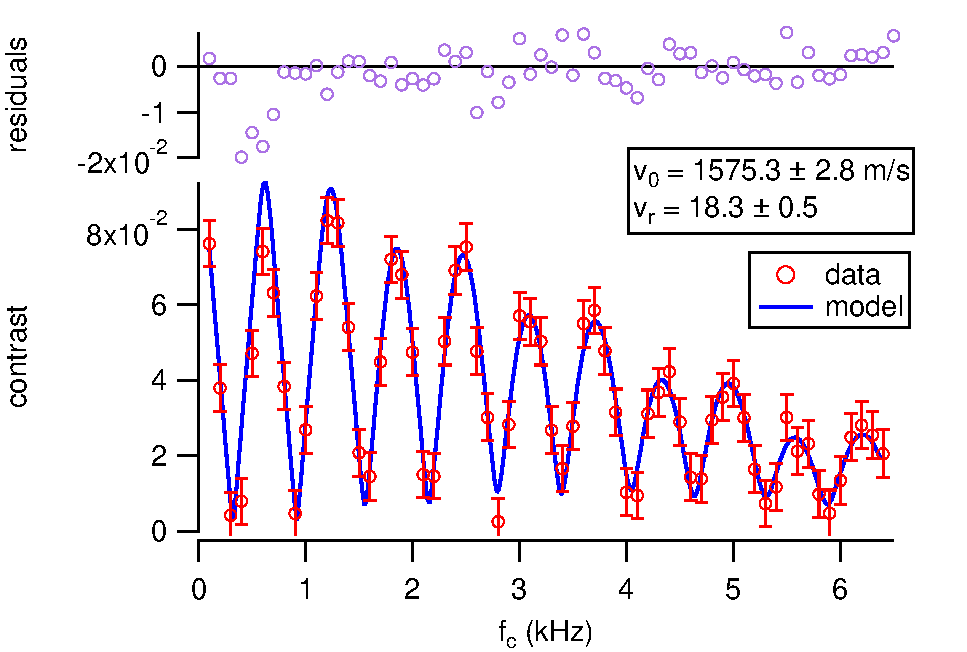
\includegraphics[width=\linewidth,keepaspectratio]{CvCF_150420_o.pdf}
\caption{\label{CvCFExample}An example of a measurement of contrast loss vs. phase chopper frequency for a Cs beam. We fit a model to these data that has $v_0$ and $v_r$ as fit parameters in order to measure the velocity distribution.}
\end{figure}
	
The uncertainty budget for velocity distribution measurement is given in \figref{velError}. The measured values of $v_0$ and $v_r$ also have statistical uncertainty in addition to uncertainty in the fit of measured $C/C_{\mathrm{ref}}(f_c)$ to the model. Uncertainty in the measurement of $\Delta\Phi = \Phi_{c1,\mathrm{on}} - \Phi_{\mathrm{ref}}$ leads to uncertainty in $A_{ci}$, which in turn propagates forward as additional uncertainty in $v_0$ and $v_r$. The total statistical uncertainty in measured $v_0$ and $v_r$ is roughly $10\times$ larger than the total systematic uncertainty.

\begin{figure}
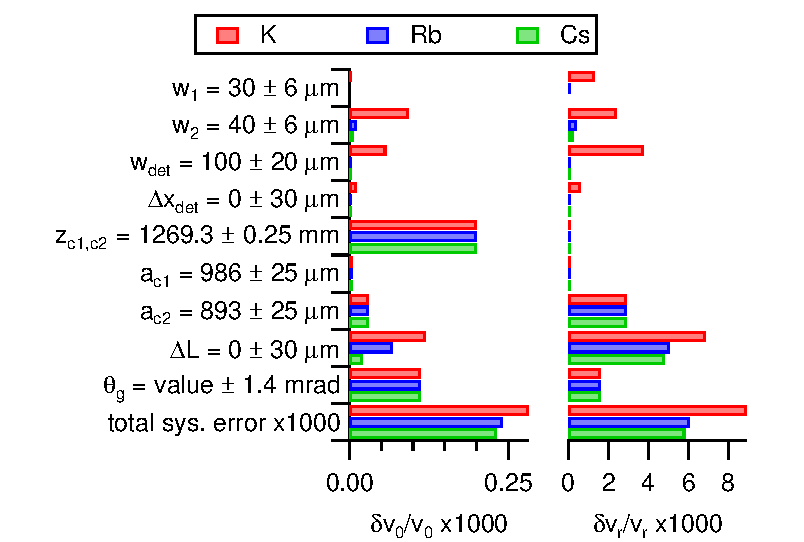
\includegraphics[width=\linewidth,keepaspectratio]{displayVelErrors.pdf}
\caption{\label{velError}Systematic uncertainty budget for measurements of $v_0$ and $v_r$ for our Cs, Rb, and K beams. Parameters $w_1$, $w_2$, and $w_{\mathrm{det}}$ are the widths of collimating slits 1 and 2 and the detector. $a_{ci}$ is the width of phase chopper $i$, and $z_{c1,c2}$ is the longitudinal distance between choppers. A nominal value for $\theta_g$ is not listed because $\theta_g$ changed from -2.37 mrad to 1.73 mrad toward the end of the experiment.}
\end{figure}

\subsection{II.c. Polarizability Measurement}

\begin{figure}
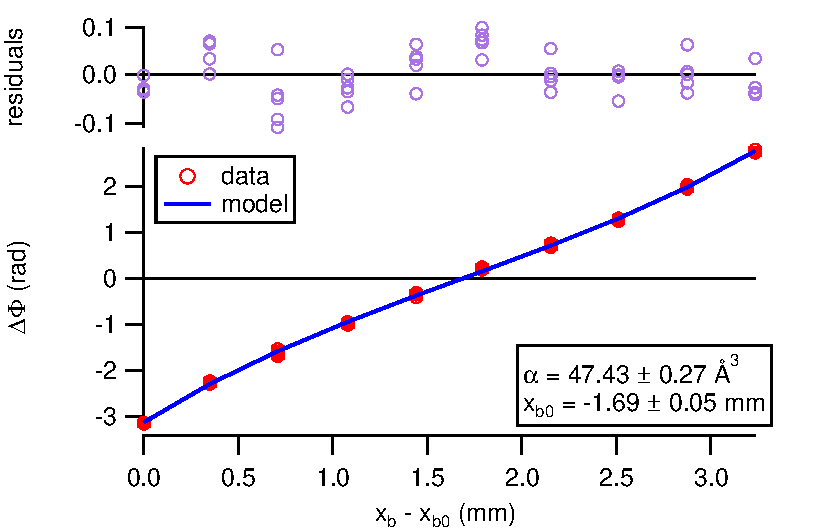
\includegraphics[width=\linewidth,keepaspectratio]{dPvMP_150327_q.pdf}
\caption{\label{dPvMPExample}An example of a measurement of phase shift vs $x$ position of the pillars for a Rb beam. The two fit parameters used to fit the model to these data are polarizability and the pillars' position at which the phase shift is null.}
\end{figure}

To measure the atoms' polarizability, we use two parallel, oppositely charged, $1/2$-inch-diameter pillars mounted to a single, rigid support structure. The pillars are mounted so that a $(3999.7 \pm 1.0)\mu$m gap exists between them. A motor moves the support structure in the $\pm x$ direction, and a length gauge monitor's the structure's $x$ position. We scan the assembly across the beam so that the beam traverses the gap between the pillars, turning the field on and off as it scans, to observe the phase shift $\Delta\Phi = \Phi_{\mathrm{pillars,on}} - \Phi_{\mathrm{ref}}$ applied by the pillars as a function $x_b$ (see an example in \figref{dPvMPExample}). $\Phi_{\mathrm{ref}}$ is once again the reference phase and contrast observed when there are no polarizing electric fields present.
When the pillars are on, we instead observe
\begin{align}
	C_{\textrm{pillars,on}}e^{\Phi_{\textrm{pillars,on}}} = 
		C_0e^{\Phi_0}		
		\frac{1}{2} \sum_{j=-1,1}
		\int_{v=0}^{\infty} P(v) \nonumber \\ \times
		e^{
			\Delta\Phi_{\vec{E},j}(v,x_b) + 
			\dphisag(v) + \dphiaccel(v) + \dphisepj(v)
		} 
		dv
	\label{CPPolesEOn}
\end{align}
We fit a model to $\Delta\Phi = \Phi_{pillars,\mathrm{on}} - \Phi_{\mathrm{ref}}$ as shown in \figref{dPvMPExample}, the fit parameters of which are $\alpha$ and the pillars position for which the phase shift is null. Because $\Delta\Phi$ vs pillars position is very linear near the zero crossing, we can determine that zero crossing to very high precision. 
This changes a previously significant systematic uncertainty, associated with measuring the distance between the beam and the physical ground plane, into an insignificant statistical uncertainty.
Additionally, being able to measure $\Delta\Phi$ on both sides of the virtual ground plane (rather than on only one side of a physical one) makes it unnecessary to consider $\dphisag$. 

\begin{figure}
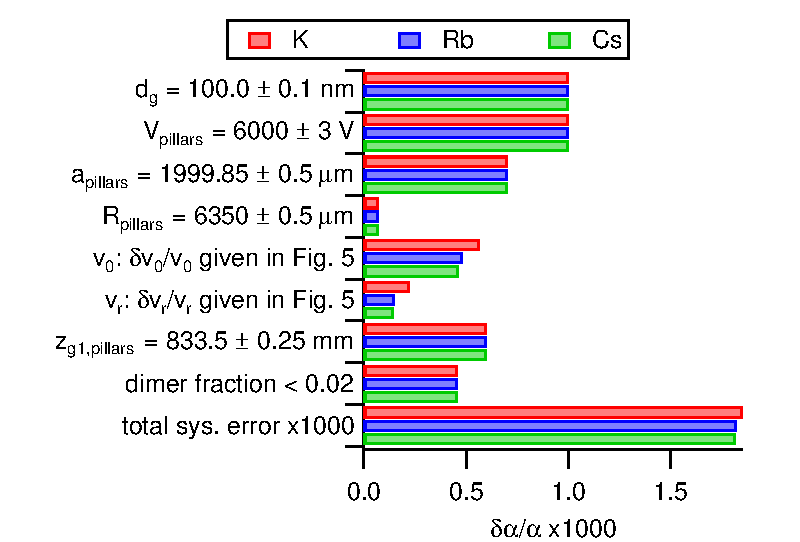
\includegraphics[width=\linewidth,keepaspectratio]{displayPolErrors.pdf}
\caption{\label{polError}(Color online) Systematic uncertainty budget for polarizability measurements for our Cs, Rb, and K beams.
The uncertainties in knowledge of $v_0$ and $v_r$ are propagated forward from \figref{velError}.}
\end{figure}

The systematic uncertainty budget for the absolute polarizability measurements is shown in \figref{polError}. We reduced some uncertainty contributions simply by measuring the apparatus geometry more carefully.
We constructed the new pillars using steel rods, the widths of which were accurately known to $1 \mu \text{m}$. This reduced the contribution to $\delta\alpha/\alpha$ from uncertainty in pillars radius by about a factor of 10.
We reduced $\delta\alpha/\alpha$ due to uncertainty in the pillars' voltage by a factor of 3 by independently calibrating our voltage supplies. We also reduced $\delta\alpha/\alpha$ due to uncertainty in distance between the pillars and the effective ground plane by sweeping the pillars across the atom beam and observing how far the pillars traveled between points at which the atom beam half-eclipsed each pillar. We were able to measure the distance between the first grating and the pillars to 1/4 mm accuracy rather than 2 mm accuracy. 

Our $\alpha$ measurements are not as strongly affected by uncertainty in $\theta_g$ as our velocity distribution measurements. To report $\alpha$ incorrectly by 0.1\%, we must use a $\theta_g$ in our polarizability data analysis that is incorrect by 23 mrad. Since both our $|\theta_g|$ and our uncertainty therein are well below that threshold, we need not consider $\dphiaccel$ in our polarizability analysis.
Also, because we set $\Delta L = 0$, we need not consider $\dphisep$.
Even if we do consider $\dphisep$, we find that our 25$\mu$m uncertainty in $\Delta L$ does not contribute significantly to uncertainty in measured $\alpha$.
Therefore, $\dphisag$, $\dphiaccel$, and $\dphisep$ are included in \eqnref{CPPolesEOn} for tutorial purposes only--our results are unaffected if we remove them.

Additionally, we found that modeling the beam's thickness and divergence was unnecessary for analysis of polarizability data if $\Delta L = 0$ and becomes increasingly important as $|\Delta L|$ increases. Because we keep $\Delta L$ close to 0, we find our reported results do not change if we model the beam's thickness and divergence.
Therefore the related parameters, $w_1$, $w_2$, $w_{\mathrm{det}}$, and $\Delta x_{\mathrm{det}}$, do not appear in the polarizability analysis error budget.

Considering second order diffraction in our model of the interferometer does not change $v$ by more than 0.05 ppt, $v_r$ by 2 ppt, and $\alpha$ by 0.1 ppt. This is primarily because the fraction of atoms in those interferometer paths is so small. Also, second-order diffraction angles are small enough so that the atoms hit the detector, then they are not sufficiently separated from the first-order interferometer paths.

\subsection{II.d. Data Analysis}

\begin{figure*}
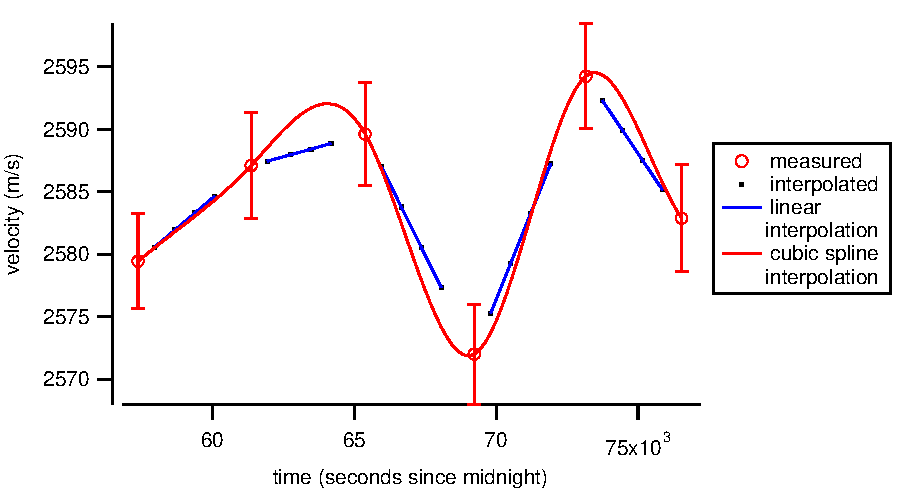
\includegraphics[width=0.49\linewidth,keepaspectratio]{velVsTime_150212.pdf}
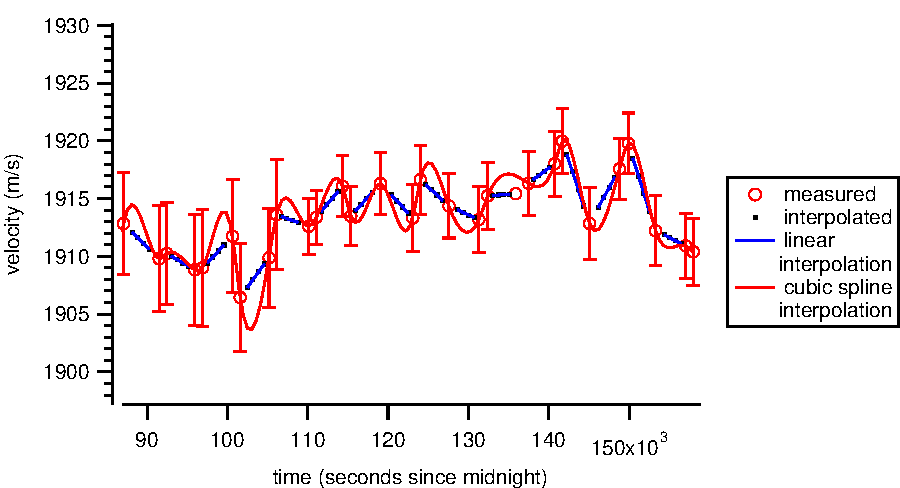
\includegraphics[width=0.49\linewidth,keepaspectratio]{velVsTime_150413.pdf}
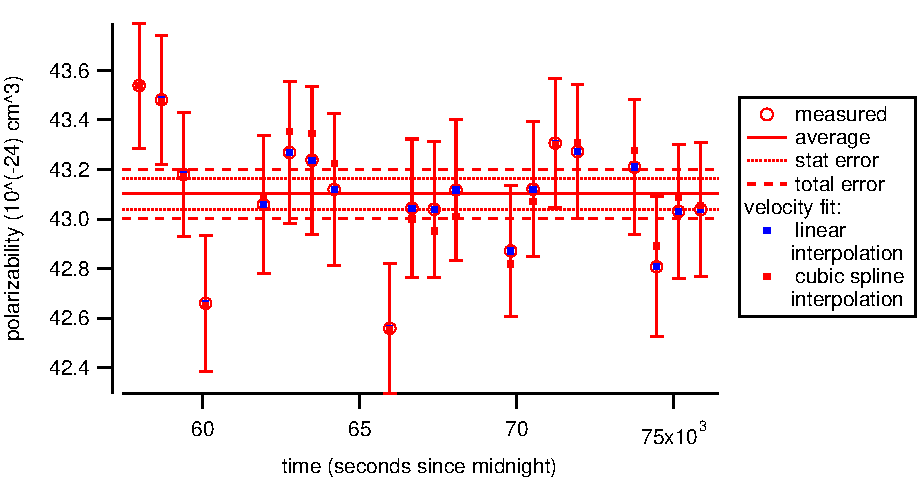
\includegraphics[width=0.49\linewidth,keepaspectratio]{polVsTime_150212.pdf}
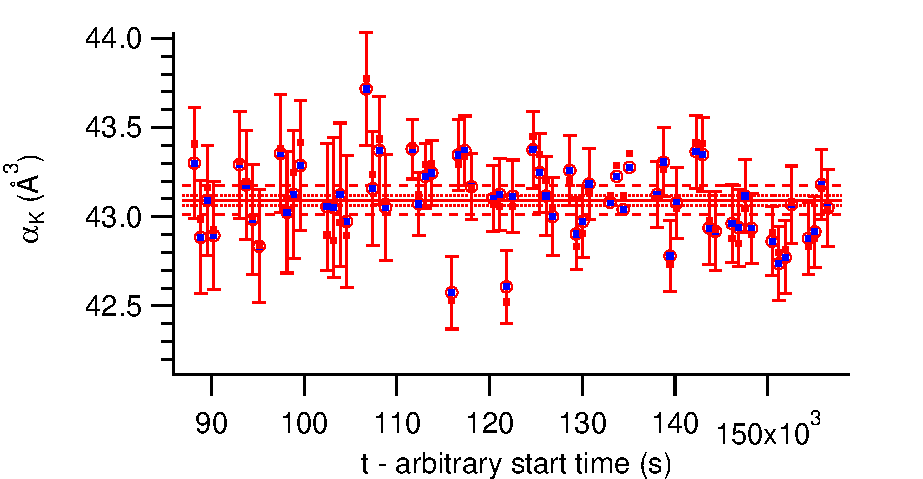
\includegraphics[width=0.49\linewidth,keepaspectratio]{polVsTime_150413.pdf}
\caption{\label{velPolVsTimeExample}(Color online) The results of $v_0$ (top) and $\ak$ (bottom) measurements taken during two different days (left and right). Both linear and cubic spline interpolations between $v_0$ measurements are reasonable, and higher differences between the two interpolations during $\ak$ measurements increase the error bars on said measurements. For these data, we chose to use linear interpolation because we believe it more accurately represents $v_0$ vs $t$--the cubic spline interpolation sometimes gains too much curviture, especially when back-to-back velocity measurements, such as those in the top-left, yield results that differ by an error bar. The red dots on the bottom graphs show what the measured $\ak$ would be if we were to use cubic spline interpolation instead. The top graphs show some typical structures that occur in $v_0$ vs time. This figure also demonstrates how we obtain the same $\ak$ for very different velocities.}
\end{figure*}

\begingroup
\begin{table}
\caption{\label{schedule}A typical sequence of measurements during a day of data acquisition. The $+x$ direction is arbitrarily chosen--the important aspect is that we spend an equal amount of time scanning the pillars in each direction so as to minimize possible systematic errors. This sequence of eight measurements is repeated for as long as we choose to acquire data. We end the data acquisition by repeating the first four measurements.}
\begin{center}
\begin{tabular}{l l}
\hline
\hline
Type of data acquired & Duration \\
\hline
contrast vs chopping freq. & 7m 5s \\
chopper 1 phase & 3m 45s \\
chopper 2 phase & 3m 45s\\
contrast vs chopping freq. & 7m 5s \\
$\Delta\Phi$ vs pillars position ($+x$ direction) & 8m 45s \\
$\Delta\Phi$ vs pillars position ($-x$ direction) & 8m 45s \\
$\Delta\Phi$ vs pillars position ($+x$ direction) & 8m 45s \\
$\Delta\Phi$ vs pillars position ($-x$ direction) & 8m 45s \\
\hline
\hline
\end{tabular}
\end{center}
\end{table}
\endgroup

A typical sequence of measurements is shown in Table \ref{schedule}.
We measure the velocity distribution twice between every four scans of the pillars across the beam, and calibrate the phase choppers between each pair of velocity measurements.
We interpolate the velocity distribution between measurements to estimate it for each pillars scan. The error bars on each interpolated $v_0$ and $v_r$ value are due to the error bars on neighboring measurements and the different ways we believe $v_0$ and $v_r$ might be reasonably interpolated. For example, we believe linear and cubic spline interpolations are reasonable, so the error bars at a given time take into account the differences between those interpolations--a larger difference between reasonable interpolations leads to larger error bars on interpolated values. That uncertainty is then propagated forward and combined with the statistical uncertainty of the fit to $\Delta\Phi$ vs $x_b$ to determine the error bars on the polarizability measurements. \figref{velPolVsTimeExample} shows an example of interpolations between $v_0$ measurements at the times of various pillars scans.

\section{III. Results and Discussion}

Table \ref{tableAbs} shows our absolute measurements of Cs, Rb, and K polarizability and their statistical and systematic uncertainties. The statistical uncertainty reported is the standard error of the mean.

\begingroup
\begin{table}
\caption{\label{tableAbs}Absolute measurements of Cs, Rb, and K static, ground-state polarizabilities.}
\begin{center}
\begin{tabular}{l l l l}
\hline\hline
Atom & avg $v_0$ (m/s) & avg $v_r$ & $\alpha$(stat.)(sys.) ($\AAA^3$) \\
\hline
Cs & 1585 & 19.8 & $\polCs$ \\
Rb & 1890 & 22.9 & $\polRb$ \\
K  & 2113 & 13.2 & $\polK$ \\
\hline\hline
\end{tabular}
\end{center}
\end{table}
\endgroup

Table \ref{tableRatio} shows our ratio measurement results. 
Even though uncertainties in $w_1$, $w_2$, $w_{\mathrm{det}}$, and $\Delta L$ contribute differently to uncertainties in measured $v_0$ and $v_r$, the total systematic uncertainty for each atom is still very similar.
Because we used the same apparatus for each absolute measurement, the systematic uncertainties mentioned in \figref{velError} and \figref{polError} are correlated for different atoms. Since those systematic uncertainties are very similar, they only barely contribute to the ratio measurement uncertanties--the ratios' statistical uncertainties are almost 20 times higher than the ratios' systematic uncertainties.
Thus we are able to achieve $< 0.1\%$ uncertainty in our measured ratios.

\begingroup
\begin{table}
\caption{\label{tableRatio}Ratio measurements of Cs, Rb, and K static, ground-state polarizabilities. The systematic errors in each ratio, which arise from the fact that the systematic errors in different measurements are not perfectly correlated, are negligible compared to the statistical errors.}
\begin{center}
\begin{tabular}{l l l}
\hline\hline
Ratio & Value(stat.) & Sys. Err. \\
\hline
$\acs/\ak$  & $\ratCsK$ & $4\cdot 10^{-5}$  \\
$\acs/\arb$ & $\ratCsRb$ & $5\cdot 10^{-6}$ \\
$\arb/\ak$  & $\ratRbK$ & $3\cdot 10^{-5}$ \\
\hline\hline
\end{tabular}
\end{center}
\end{table}
\endgroup

\subsection{III.a. Comparisons With Other Experimental and Theoretical Polarizabilities}

\begin{figure*}
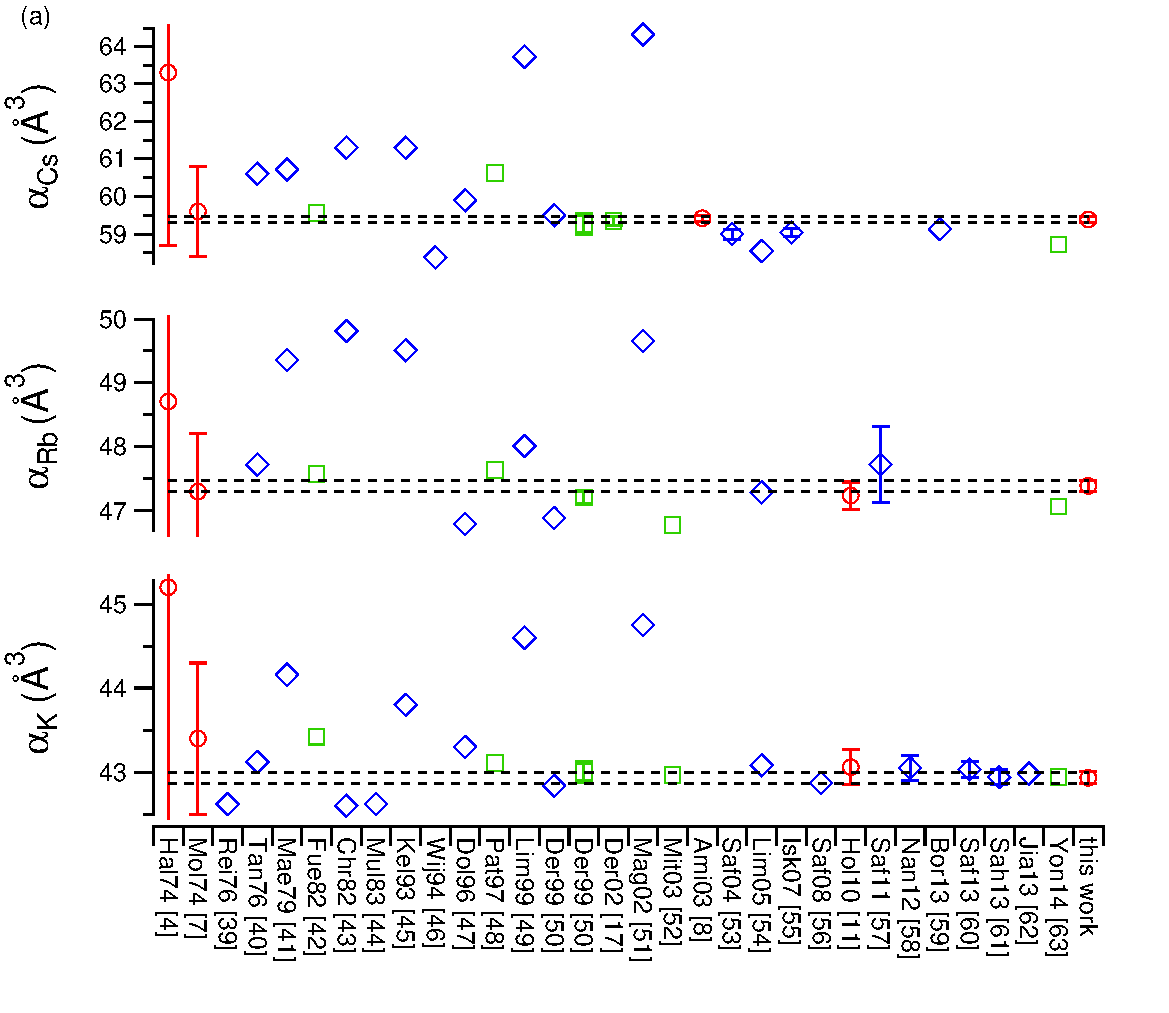
\includegraphics[width=0.60\linewidth,keepaspectratio]{displayAbsComps.pdf}
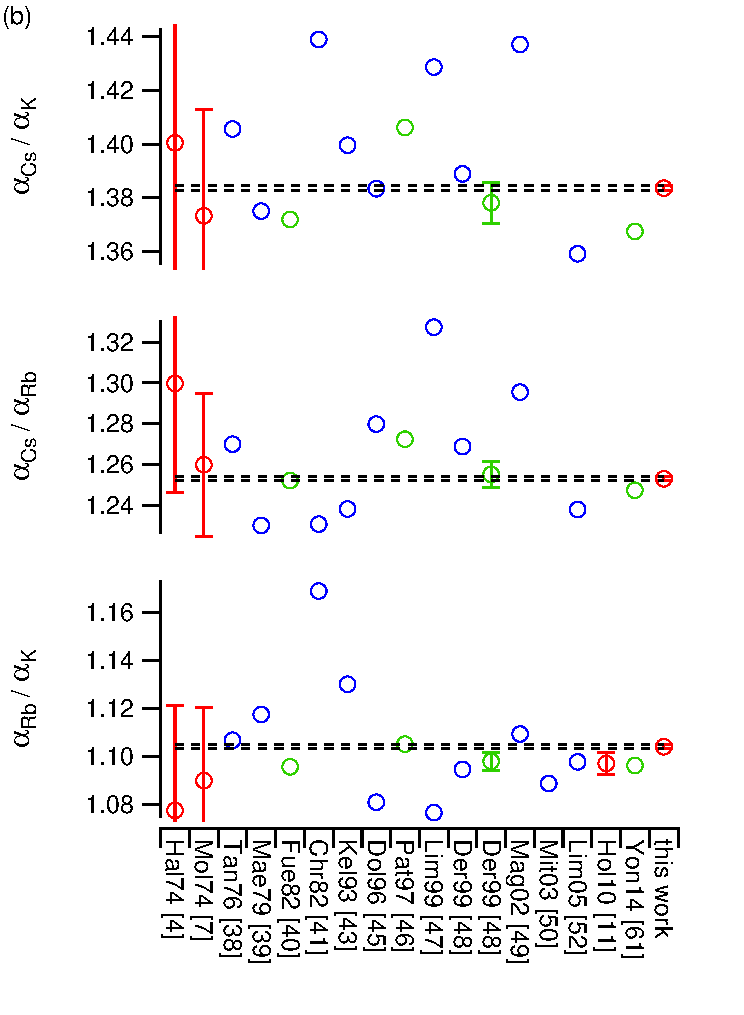
\includegraphics[width=0.38\linewidth,keepaspectratio]{displayRatComps.pdf}

\includegraphics[width=0.55\linewidth,keepaspectratio]{displayCompsLegend.pdf}
\caption{\label{comparisons}(Color online) Our absolute measurements (left) and ratio measurements (right) compared with other measurements, \textit{ab initio} calculations, and semi-empirical calculations 
\cite{Molof1974,Hall1974,Tang1976,Reinsch1976,Kutzelnigg1978,
Christiansen1982,Fuentealba1999,Muller1984,Kello1993,VanWijngaarden1994,
Dolg1996,Patil1997,Derevianko1998,Magnier2002,Derevianko2001,
Amini2003,Mitroy2003,Safronova2004,Lim2005,Safronova2008,
Holmgren2010,Safronova2011,Nandy2012,Jiang2013,Sahoo2013,
Safronova2013,Borschevsky2013,Y.-B.2014}.
The references are represented on the x-axis by the first three letters of the first author's last name followed by the year of publication. For the semi-empirical calculations: Reference Fue82 used semi-empirical pseudopotentials \cite{Fuentealba1999}, Pat97 used experimentally-determined energy levels \cite{Patil1997}, Der99 used experimentally-determined electric dipole transition matrix elements \cite{Derevianko1998}, and Yon14 used semi-empirical core polarization potentials \cite{Y.-B.2014}.}.
\end{figure*}

\begin{figure}
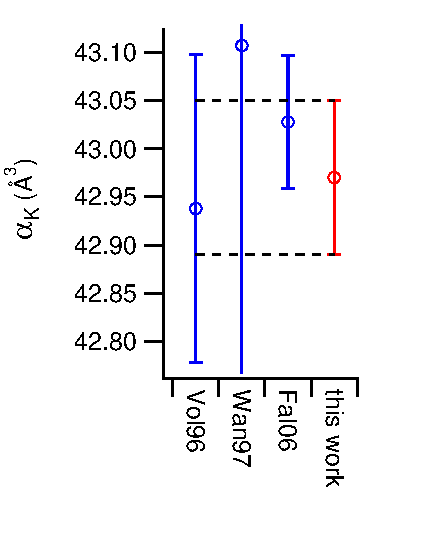
\includegraphics[width=0.49\linewidth,keepaspectratio,valign=t]{displayKMisc.pdf}
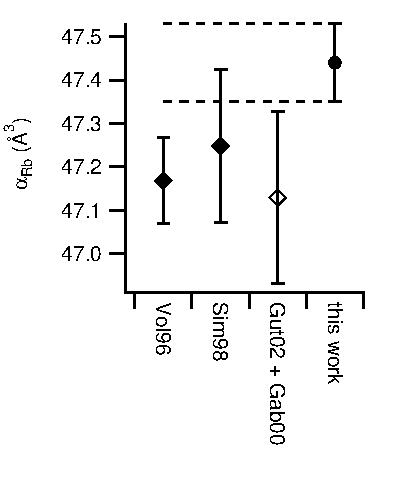
\includegraphics[width=0.49\linewidth,keepaspectratio,valign=t]{displayRbMisc.pdf}
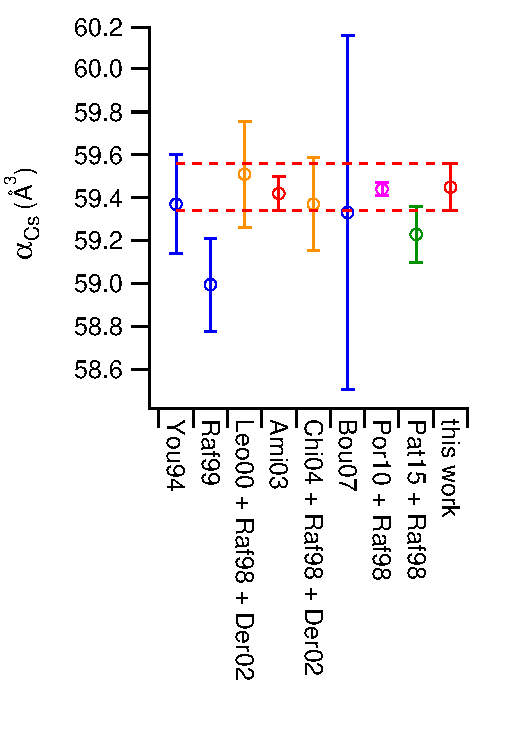
\includegraphics[width=0.620\linewidth,keepaspectratio,valign=t]{displayCsMisc.pdf}
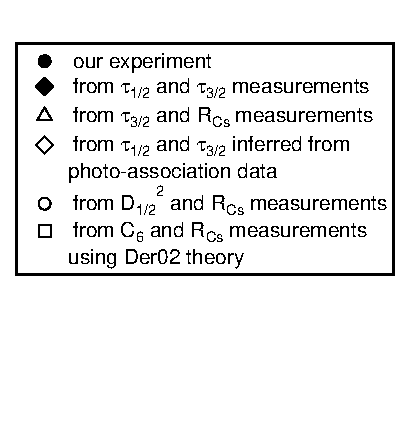
\includegraphics[width=0.365\linewidth,keepaspectratio,valign=t]{displayMiscLegend.pdf}
\caption{\label{comparisonsMisc}(Color online) Comparisons of our measured polarizabilities and Amini and Gould's $\acs$ measurement \cite{Amini2003} to polarizabilities derived from measured lifetimes and lifetime ratios,
\cite{Young1994,Rafac1999,Bouloufa2007,Falke2006a,Volz2006,Simsarian1998,Wang1997,Rafac1998}, 
lifetimes inferred from photo-association data
\cite{Gabbanini2000,Gutterres2002},
theoretical $D^2$ values
\cite{Porsev2010},
and van der Waals $C_6$ measurements
\cite{Leo2000,Chin2004,Derevianko2001}.}
\end{figure}

\figref{comparisons} compares our polarizability measurements with theoretical calculations, semi-empirical calculations, and experimental measurements subsequent to and including Molof \etal's and Hall \etal's 1974 measurements \cite{Molof1974,Hall1974}. Our absolute measurements are consistent with all previous absolute measurements. 
In particular, our $\acs$ measurement agrees very well with Amini and Gould's recent $\acs$ measurement (shown again in \figref{comparisonsMisc}) \cite{Amini2003}. Amini and Gould's $\acs$ measurement, in addition to being dramatic improvement in precision since the previous measurement by Molof \etalspace \cite{Molof1974}, is the only polarizability measurement using the fountain method. The fact that we obtained a very similar $\acs$ as Amini and Gould with a very different apparatus goes a long way toward validating both methods.

\figref{comparisons} also compares our ratios to other theoretical, semi-empirical, and experimental ratios. Our ratios are also consistent with all previous ratio measurements.

\subsection{III.b. Comparisons With Polarizabilities Derived From Other Quantities}

Static polarizabilities can be related to electric dipole transition matrix elements, state lifetimes, oscillator strengths, and van der Waals coefficients. We will describe those relations and compare our $\alpha$ measurements to $\alpha$ values derived from recent calculations and high-precision measurements of those quantities; those comparisons are shown in \figref{comparisonsMisc}.

\begingroup
\begin{table}
\caption{\label{tableCoreTail}We use the following core polarizabilities ($\acore$) and tail polarizabilities ($\atail$) in order to derive polarizabilities from lifetime measurements and matrix elements from polarizabilities. The sources are cited next to each value in the table. We acknowledge that there are several recent theoretical $\acore$ values for 
Cs \cite{Sansonetti1981,Johnson1983,Safronova1999,Derevianko2001}, 
Rb \cite{Johnson1983,Safronova1999}, and 
K \cite{Johnson1983,Muller1984}
that vary by up to 0.03\%, 0.07\%, and 0.4\% of $\alpha$, respectively.}
\begin{center}
\begin{tabular}{l l l}
\hline\hline
Atom & $\acore (\AAA^3)$ & $\atail (\AAA^3)$ \\
\hline
Cs & 2.34 \cite{Lim2002} & 0.16 \cite{Derevianko2001} \\
Rb & 1.36 \cite{Lim2002} & 0.15 \cite{Safronova2011} \\
K  & 0.82 \cite{Lim2002} & 0.11 \cite{Sahoo2013} \\
\hline\hline
\end{tabular}
\end{center}
\end{table}
\endgroup

The polarizability (in volume units) of an atom in state $i$ can be written in terms of state lifetimes as
\begin{align}
	\alpha_i = \frac{3c^3}{2} \sum_{k\neq i} 
	\frac{1}{\tau_{ki} \omega_{ik}^4} \frac{g_k}{3g_i}
	+ \acore
	+ \atail
	\label{polFromLifetimes}
\end{align}
where $\tau_{ki}$ is the lifetime associated with spontaneous decay from state $k$ to $i$, $\omega_{ik}$ is the transition frequency between states $i$ and $k$, and $g_n = 2J_n+1$ is the degeneracy factor for state $n$. In our case, state $i$ is the ground state. $\acore$ is the polarizability of the core electrons, and $\atail$ approximates all the terms not explicitly included in the sum; we only explicitly consider $Ns_{1/2}-Np_{1/2}$ and $Ns_{1/2}-Np_{3/2}$ transitions, where $N=6$ for Cs, $N=5$ for Rb, and $N=4$ for K. 
We abbreviate the lifetimes associated with those transitions to $\tau_{1/2}$ and $\tau_{3/2}$.
In our calculations, we use the $\acore$ and $\atail$ values indicated in Table \ref{tableCoreTail}.
The $\omega_{0k}$ values are calculated using transition wavelengths reported by NIST \cite{NIST}. 
\figref{comparisonsMisc} shows polarizabilities calculated using measurements of $\tau_{1/2}$ and $\tau_{3/2}$
\cite{Young1994,Rafac1999,Bouloufa2007,Falke2006a,Volz2006,Simsarian1998,Wang1997}.
\figref{comparisonsMisc} also shows $\acs$ calculated from 
values of $\tau_{1/2,\mathrm{Rb}}$ and $\tau_{3/2,\mathrm{Rb}}$ inferred in 2002 by Gutterres \etalspace from photo-association data taken in 2000 by Gabbanini \etalspace \cite{Gabbanini2000,Gutterres2002}.
Additionally, Rafac and Tanner measured the ratio of Cs electric dipole transition matrix elements
\begin{align}
	\rcs = \frac
	{\left|\brakett{6s_{1/2}}{\hat{D}}{6p_{3/2}}\right|^2}
	{\left|\brakett{6s_{1/2}}{\hat{D}}{6p_{1/2}}\right|^2}
	\label{polFromLifetimes}
\end{align}
which we can use to deduce a ratio of lifetimes
\begin{align}
	\frac{\tau_{1/2}}{\tau_{3/2}} = \frac{R_{Cs}}{2} \left( \frac{\omega_{3/2}}{\omega_{1/2}} \right)^3
	\label{RafacRLifetimes}
\end{align}
We can use this lifetimes ratio with Patterson \etal's 2015 measurement of $\tau_{3/2,\mathrm{Cs}}$ to report $\acs$ \cite{Patterson2015}.

We can write $\alpha_i$ in terms of the electric dipole transition matrix elements as
\begin{align}
	\alpha_i = \frac{e^2}{12 \pi \epsilon_0 a_0^4} \sum_{k\neq i}	
	\frac{\left|\brakett{i}{\hat{D}}{k}\right|^2}{\hbar\omega_{ik}}	
	+ \acore
	+ \atail
	\label{polFromMatrixElements}
\end{align}
where $a_0$ is the Bohr radius. 
As before, we only explicitly consider the $Ns_{1/2}-Np_{1/2}$ and $Ns_{1/2}-Np_{3/2}$ matrix elements, 
where $Ns_{1/2}$ is the ground state.
We use $\rcs$ along with Porsev \etal's 2010 calculation of $D_{1/2,\mathrm{Cs}}^2 = 20.334$ (in atomic units) to report polarizability \cite{Rafac1998,Porsev2010}.

In 2002, Derevianko and Porsev demonstrated a method for obtaining values of $D_{1/2,\mathrm{Cs}}^2$ from Cs van der Waals $C_6$ coefficients \cite{Derevianko2001}. \figref{comparisonsMisc} includes $\alpha$ values derived using experimental Cs $C_6$ measurements in conjunction with Derevianko and Porsev's method and $\rcs$ \cite{Leo2000,Chin2004,Derevianko2001,Rafac1998}.

\subsection{III.c. Other Atomic Properties Derived From Our Polarizability Measurements}

Finally, we use our polarizability measurements along with $\rcs$ and the $\acore$ and $\atail$ values from Table \ref{tableCoreTail} to report matrix elements $|D|$, lifetimes, oscillator strengths, and line strengths. To report matrix elements and lifetimes, we use \eqnref{polFromMatrixElements} and \eqnref{polFromLifetimes}. $\alpha_i$ is given in terms of oscillator strengths $f_{ik}$ as 
\begin{align}
	\alpha_i = \frac{e^2}{4 \pi \epsilon_0 m}
	\sum_{k \neq i}
	\frac{f_{ik}}{w_{ik}^2}
	+ \acore
	+ \atail
	\label{polFromOscStr}
\end{align}
where $m$ is the electron mass. 
$\alpha_i$ is also given in terms of line strengths as
\begin{align}
	\alpha_i = \frac{1}{6\pi\epsilon_0\hbar} 
	\sum_{k \neq i} 
	\frac{S_{ki}}{g_i\omega_{ik}}
	+ \acore
	+ \atail
	\label{polFromLineStr}
\end{align}
Additionally, we use Derevianko and Porsev's method to report a Cs van der Waals $C_6$ coefficient. These results are displayed in Table \ref{tableMisc}. We note that our $\left|D_{1/2,\mathrm{Cs}}\right|$ value agrees very well with the theoretical $\left|D_{1/2,\mathrm{Cs}}\right|$ calculated by Porsev \etalspace in 2010 for the purpose of interpreting PNC data \cite{Porsev2010}.

We can also use our measurements together with recent measurements of Cs, Rb, and K $\alpha_{Np_{1/2}} - \alpha_{Ns_{1/2}}$ \cite{Hunter1991,Miller1994} to report excited state polarizabilities $\alpha_{Np_{1/2}}$. 
These results are also shown in Table \ref{tableMisc}.

\begingroup
\begin{table}
\caption{\label{tableMisc}Matrix elements, lifetimes, oscillator strengths, and van der Waals $C_6$ coefficients calculated from our polarizability measurements along with Rafac and Tanner's $R_{\mathrm{Cs}}$ \cite{Rafac1998}. The $C_6$ coefficient was calculated using Derevianko and Porsev's method of obtaining $C_6$ from matrix elements \cite{Derevianko2001}. The matrix elements, line strengths, and $C_6$ coefficient are expressed in atomic units, while the lifetimes are expressed in SI units. In the last row heading, $N=6$ for Cs, $N=5$ for Rb, and $N=4$ for K.}
\begin{center}
\begin{tabular}{l l l l}
\hline\hline
Quantity & Cs & Rb & K \\
\hline
$\left|D_{1/2}\right|$	& 4.510(4) & 4.255(4) & 4.116(4) \\
$\left|D_{3/2}\right|$	& 6.347(6) & 5.989(6) & 5.793(6) \\
$\tau_{1/2}$ (ns)		& 34.75(6) & 27.39(5) & 26.61(5) \\
$\tau_{3/2}$ (ns)		& 30.34(6) & 26.15(5) & 26.51(5) \\
$f_{1/2}$				& 0.3453(6) & 0.3459(7) & 0.3342(6) \\
$f_{3/2}$				& 0.7179(14) & 0.6981(14) & 0.6649(13) \\
$S_{1/2}$ 				& 20.34(4) & 18.11(5) & 16.94(3) \\
$S_{3/2}$ 				& 40.29(8) & 35.87(7) & 33.56(6) \\
$C_6$					& 6877(23) & & \\
$\alpha_{Np_{1/2}}$ ($\AAA^3$)		& 196.87(11) & 120.38(9) & 89.96(8) \\
\hline\hline
\end{tabular}
\end{center}
\end{table}
\endgroup

\section{IV. Outlook}

We are currently exploring ways to measure the polarizability of either Li or metastable He, the polarizabilities of which can be easily calculated. By measuring $\acs/\alpha_{\mathrm{He*}}$ or $\acs/\alpha_{\mathrm{Li}}$, we could report an absolute measurement of $\acs$ with precision comparable to that of the ratios reported here for the benefit of PNC research. Such a measurement would also act as a calibration of the measurements presented in this work, because it would be independent of systematic errors that may affect our absolute measurements.

We are also exploring electron-impact ionization schemes for atom detection, which would allow us to detect a much broader range of atoms and molecules. Our Langmuir-Taylor only allows us to detect alkali metals and some alkaline-Earth metals. Installing a new, "universal" detector would allow us to broaden the scope of atom interferometry as a precision measurement tool. 

This work is supported by NSF Grant No. 1306308 and a NIST PMG. M.D.G. and R.T. are grateful for NSF GRFP Grant No. DGE-1143953 for support. 


%\bibliography{references}
\bibliography{library}

\end{document}  